\documentclass{article}
\usepackage{amsmath}
\usepackage{graphicx}
\usepackage{float}
\usepackage{geometry}
\usepackage{hyperref}
\usepackage{calc}
\usepackage{enumitem}
\usepackage{color}
\usepackage{adjustbox}
\usepackage{xcolor}
\hypersetup{
    colorlinks,
    linkcolor={red!50!black},
    citecolor={blue!50!black},
    urlcolor={blue!80!black}
}
\usepackage{xepersian}
\settextfont[
    Scale = 1.3 ,
    BoldFont = *Bd ,
    ItalicFont = *It ,
    Extension = .ttf
]{XB Niloofar}
\AddEnumerateCounter{\alph}{\@alph}{\faalph}

\geometry{
    left=20mm,
    right=20mm,
    top=20mm,
    bottom=20mm,
}


\begin{document}
\begin{titlepage}
    \begin{center}
        \textbf{\Huge{گزارش آزمایش سوم آزمایشگاه
        \\ طراحی سیستم دیجیتال}}\\
        \vspace{1cm}
        
\includegraphics[width=0.3\textwidth]{sharif.jpg}\\
        \vspace{1cm}
        \textbf{ \Large{مزدک تیموریان}}\\
        \vspace{0.4cm}
        \textbf{ \large{401101495}}\\
        \vspace{0.5cm}
        \textbf{ \Large{مریم شیران}}\\
        \vspace{0.4cm}
        \textbf{ \large{400109446}}\\
        \vspace{0.5cm}
        \textbf{ \Large{مهدی بهرامیان}}\\
        \vspace{0.4cm}
        \textbf{ \large{401171593}}\\
        \vspace{1cm}
        \textbf{ \Large{دانشکده مهندسی کامپیوتر}}\\
        \vspace{0.4cm}
        \textbf{ \Large{دانشگاه صنعتی شریف}}\\
        \vspace{0.6cm}
        \large{تیر 1403}
    \end{center}
    \thispagestyle{empty}
\end{titlepage}

\tableofcontents

\newpage

\section{شرح آزمایش}

\subsection{مقایسه کننده ۱ بیتی آبشاری}

این مقایسه کننده به این صورت کار میکند که وضعیت رقم های بزرگتر را میگیرد
و اگر در آن رقوم دو عدد برابر بودند، خروجی برابر با نتیجه مقایسه دو رقم 
کنونی میشود و در غیر این صورت خروجی برابر با مقایسه رقوم بزرگتر میشود.

\begin{figure}[H]
    \centering
    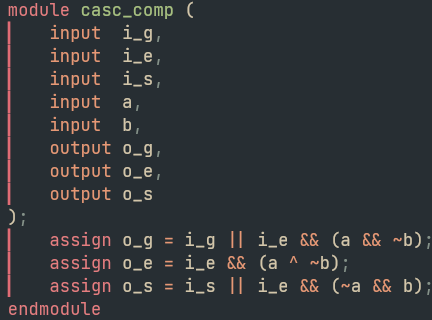
\includegraphics[width=0.6\textwidth]{./casc_comp.png}
\end{figure}
همانطور که در کد وریلاگ بالا میبینید، این عملکرد با استفاده از عملگر های
ساده منطقی پیاده سازی شده است.

\subsection{مقایسه کننده ۴ بیتی}

برای مقایسه کردن دو عدد ۴ رقمی کافیست ۴ مقایسه کننده آبشاری را پشت یکدیگر
بگذاریم و حالت اولی را با تساوی شروع کنیم.

\begin{figure}[H]
    \centering
    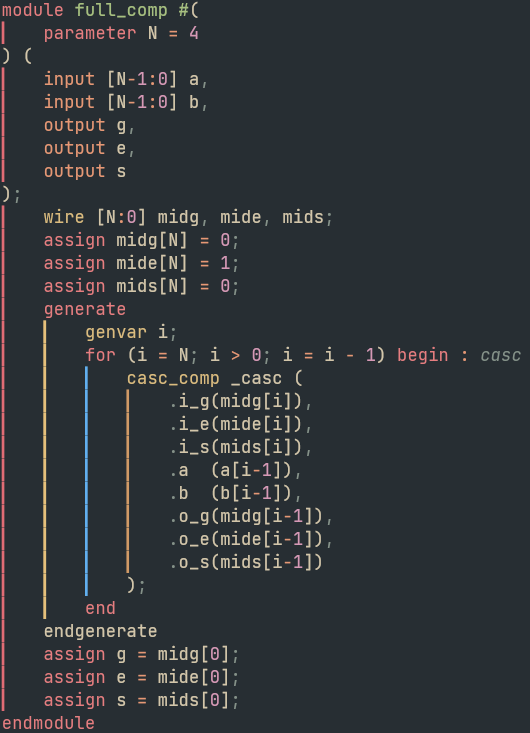
\includegraphics[width=0.6\textwidth]{./full_comp.png}
\end{figure}

همانطور که در کد وریلاگ بالا مشاهده میکنید، این عملکرد با استفاده از یک
بلوک generate پیاده سازی شده است.


\subsection{مقایسه کننده سریالی}

برای مقایسه کردن دو عدد سریالی کافیست برای وضعیت مقایسه دو عدد تا کنون 
۳
ثبات نگهداریم که این ثبات ها را میتوان با استفاده از تکنیک
\LR{master-slave}
طراحی کنیم.
سپس آنها را به ورودی مقایسه کننده آبشاری بدهیم و خروجی آنرا به ورودی 
ثبات ها و خروجی کلی مدارمان وصل کنیم.

\begin{figure}[H]
    \centering
    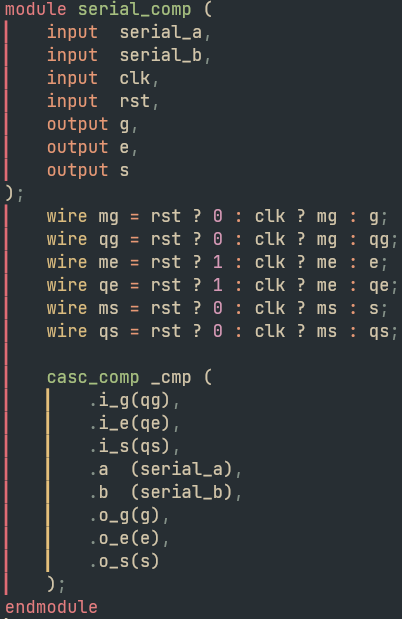
\includegraphics[width=0.6\textwidth]{./serial_comp.png}
\end{figure}

به طور کلی توصیف ما به صورت کد وریلاگ بالا قابل پیاده سازی است.

\section{شبیه سازی و بررسی عملکرد مقایسه کننده ها}


\subsection{مقایسه کننده ۴ بیتی}

برای آزمون کارایی این مدار کافیست در یک تست-بنچ ورودی های مختلفی را به مدار داد
و رفتار مدار را آزمود.

\begin{figure}[H]
    \centering
    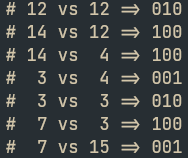
\includegraphics[width=0.3\textwidth]{./test_res.png}
\end{figure}

همانطور که در نتیجه اجرای تست بنچ میبینید، نتیجه این مقایسه ها به درستی محاسبه شده اند.
(
معنی بیت ها به ترتیب : 
$a > b | a = b | a < b$
)

\subsection{مقایسه کننده سریالی}
برای آزمایش مقایسه کننده سریالی کافیست تعدادی دفعه مدار را ریست کنیم و
سپس در هر مرحله ورودی های مورد نظر را به صورت رقم به رقم، هر رقم در یک کلاک وارد میکنیم.
در این صورت انتظار میرود که عملکرد مدار به این صورت باشد که اولین کلاکی که 
ورودی ها متفاوت بودند، نتیجه مقایسه را تعیین کند.

\begin{figure}[H]
    \centering
    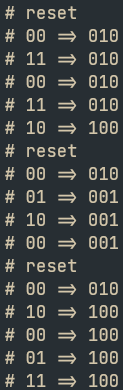
\includegraphics[width=0.2\textwidth]{./serial_test_res.png}
\end{figure}

همانطور که میبینید عملکرد مدار در این ۳ آزمون درست بوده است.

\end{document}
